\subsection{Group Collaborameter}
A Collaborameter is a serious of statements about how the group works. The statements are rated from one to five by each group memeber. One being highly disagree, and five being highly agree. The statements are all positive, so the higher the score, the more satisfied the person is with the group work. The statements are rated three times during the project. Once in the beginning, once in the middle, and one in the end. 

The first time the Collaborameter was filled out, some of the statements felt irrelevant. There are statements about having distinct goals, and about how the group solves problems. Which at this point, we had no idea about which goals to set, and did not have any problems to solve. The result from the first Collaborameter is showed in figure \ref{fig:1analysisCollaborameter}.

\begin{figure}
\centering
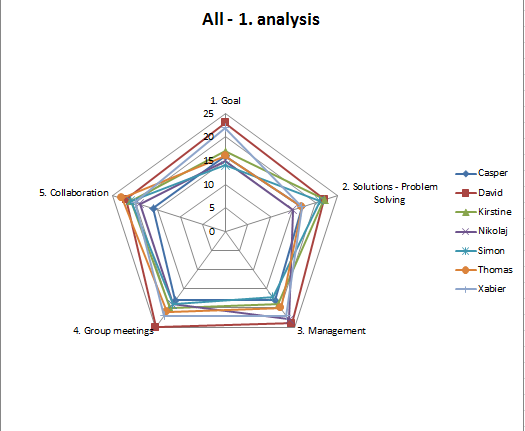
\includegraphics[width=0.7\linewidth]{graphics/1analysisCollaborameter}
\caption[Result from first Collaborameter analysis]{The result from the first Collaborameter analysis. Each person has a color. The further the color is from the center of the spiderweb, the more satisfied the person is with the groupwork.}
\label{fig:1analysisCollaborameter}
\end{figure}


The second analysis was taken more in the end of the project, than in the middle. The reason for this is that it took us a while to get started, so it felt like it was more in the middle, than the calender would say. Also, there were many things which needed to be done, and noone had focus on remembering the Collaborameter. At this time, all the goals should be clear, and everyone should know how they think the group functions. The result from the second test is in figure \ref{fig:2analysisCollaborameter}.

\begin{figure}
\centering
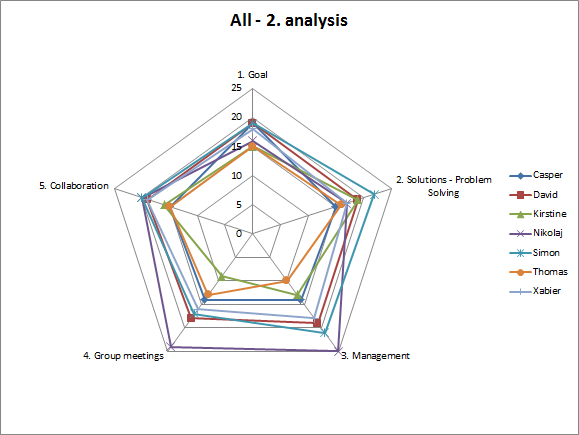
\includegraphics[width=0.7\linewidth]{./graphics/2analysisCollaborameter}
\caption{The result from the second Collaborameter analysis.}
\label{fig:2analysisCollaborameter}
\end{figure}

The third Collaborameter analysis was done in the end of the project, when almost all the goals should be fulfilled, and then everyone think the group has worked to solve the problem. The result from the third Collaborameter analysis is in figure \ref{fig:3analysisCollaborameter}.

\begin{figure}
\centering
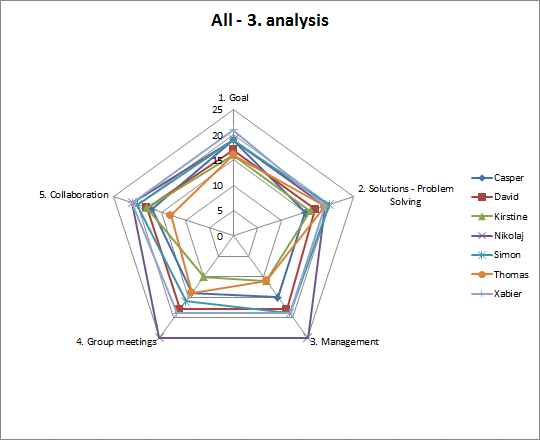
\includegraphics[width=0.7\linewidth]{./graphics/3analysisCollaborameter}
\caption{The result from the third Collaborameter analysis.}
\label{fig:3analysisCollaborameter}
\end{figure}

The three figures of the Collaborameter results show that the members of the group disagrees about how well the group is functioning. The disagreement is highest in the Group Meetings and the Management sections, and the disagreement increases throughout the project. To test how the rating of the Collaborameter statements changes throughout the project the average of the members Collaborameter ratings of the three analysis are found and shown in figure \ref{fig:ALLanalysisCollaborameter}. It is clear that the Goal categori is the one that changes the least, and the Group meeting is the one that changes the most. All the ratings are most positive in the first analysis, and then becomes more negative. The second and thirs analysis are almost the same. This is due to the short period of time between the ratings. 
\begin{figure}
\centering
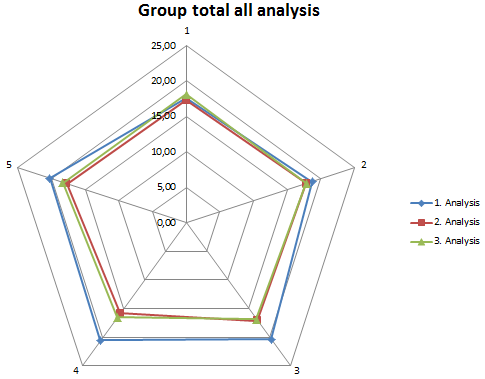
\includegraphics[width=0.7\linewidth]{./graphics/ALLanalysisCollaborameter}
\caption[Average result of the Collaborameter results]{The average result from the three Collaborameter analysis. The progress of the group work can be seen.}
\label{fig:ALLanalysisCollaborameter}
\end{figure}

